\documentclass[11pt]{article}
\usepackage[margin=1in]{geometry}
\usepackage{amsmath,amssymb}
\usepackage{graphicx}
\usepackage{booktabs}
\usepackage{hyperref}
\usepackage{natbib}
\usepackage{caption}
\usepackage{subcaption}
\usepackage{algorithm}
\usepackage{algorithmic}

\title{GlucoSim: Gymnasium Environments for Reinforcement Learning\\in Glucose Management}
\author{Hass Dhia\\Smart Technology Investments Research Institute\\partners@smarttechinvest.com}
\date{March 2026}

\begin{document}
\maketitle

% ========================================================================
\begin{abstract}
We present GlucoSim, an open-source platform providing three Gymnasium-compatible reinforcement learning environments for Type 1 diabetes glucose management: basal rate optimization (BasalControl), meal bolus dosing (BolusAdvisor), and full closed-loop insulin delivery (ClosedLoop). GlucoSim implements the Bergman minimal glucose-insulin model with RK4 integration and verified equilibrium at basal conditions, a Dalla Man two-compartment gut absorption model, a CGM sensor noise model with configurable lag and noise, and a virtual patient generator producing 30 patients across three age groups with $\pm$20\% parameter variability. We train PPO agents against random and clinical heuristic baselines across three difficulty levels and three patient age groups, organized into a five-tier benchmark suite. PPO outperforms random baselines on all three environments with increasing advantage: BasalControl (921.5 vs. 74.3 mean reward), BolusAdvisor (1101.6 vs. $-$40.7), and ClosedLoop (1822.5 vs. $-$3324.3). The difficulty gradient from basal through closed-loop creates progressively stronger separation between learned and naive policies. GlucoSim ships with 117 tests, trained PPO baselines, and is available on PyPI and GitHub under the MIT license.
\end{abstract}

% ========================================================================
\section{Introduction}

Type 1 diabetes affects over 8.4 million people worldwide and requires continuous exogenous insulin delivery to maintain blood glucose within the target range of 70--180 mg/dL~\citep{kovatchev2009silico}. Automated insulin delivery (AID) systems, commonly called artificial pancreas systems, use control algorithms to adjust insulin pump delivery based on continuous glucose monitor (CGM) readings~\citep{hovorka2004nonlinear}.

Reinforcement learning (RL) has emerged as a promising approach for insulin dosing because the problem is inherently sequential: at each time step, a controller observes glucose and decides an insulin delivery rate, receiving a reward based on glycemic outcomes~\citep{fox2020deep, zhu2020basal}. However, the field lacks standardized Gymnasium-compatible benchmarks that would allow systematic comparison of RL algorithms under controlled conditions.

Existing simulators such as simglucose~\citep{xie2018simglucose} use the older OpenAI Gym API, and GluCoEnv~\citep{hettiarachchi2022glucoenv} provides a single environment type. Neither offers a comprehensive benchmark suite with multiple environment paradigms, difficulty tiers, and clinical heuristic baselines.

GlucoSim addresses this gap with three contributions:
\begin{enumerate}
    \item Three Gymnasium-compatible environments spanning basal control, bolus dosing, and full closed-loop delivery, each with easy/medium/hard difficulty tiers and three patient age groups.
    \item A modular simulation stack combining the Bergman minimal model~\citep{bergman1979quantitative}, Dalla Man gut absorption~\citep{dallaman2007meal}, CGM sensor noise, and 30 virtual patients with realistic inter-patient variability.
    \item An empirical demonstration that model equilibrium correctness is essential for valid RL benchmarking, with PPO outperforming random on all environments when the Bergman model is properly parameterized, and a difficulty gradient that increases from basal through closed-loop control.
\end{enumerate}

% ========================================================================
\section{Related Work}

The UVA/Padova simulator~\citep{dallaman2014uvapadova} is the gold standard for in-silico glucose control research, having been accepted by the FDA as a substitute for pre-clinical animal trials. However, it is proprietary and not available as open-source software. Xie's simglucose~\citep{xie2018simglucose} implements the 2008 version of the UVA/Padova model as an open-source Python package with an OpenAI Gym interface, but uses the deprecated Gym v0.10 API and has not been updated since 2018.

Recent RL approaches to glucose control include deep Q-learning for closed-loop control~\citep{fox2020deep}, PPO-based basal rate optimization~\citep{zhu2020basal}, and bolus advisor systems using deep RL~\citep{lee2020insulin}. Ngo et al.~\citep{ngo2025safe} introduced safety constraints through dual safety mechanisms in a PPO-based controller, achieving 87.45\% median time-in-range.

Hettiarachchi et al.~\citep{hettiarachchi2022glucoenv} proposed GluCoEnv as a Gymnasium-compatible glucose control environment, but it focuses on a single control paradigm and does not provide benchmark tiers or clinical heuristic baselines for systematic comparison.

Unlike these prior works, GlucoSim provides a unified platform with three distinct control paradigms (basal, bolus, closed-loop), configurable difficulty through patient variability and meal randomization, clinical heuristic baselines, and a standardized benchmark suite -- all under the modern Gymnasium API compatible with Stable Baselines3.

% ========================================================================
\section{System Architecture}

GlucoSim implements a modular simulation stack where each component can be independently configured or replaced (Figure~\ref{fig:architecture}).

\begin{figure}[h]
\centering
\fbox{\parbox{0.9\textwidth}{
\centering
\textbf{GlucoSim Architecture}\\[6pt]
\texttt{Virtual Patient} $\rightarrow$ \texttt{Bergman Model} $\rightarrow$ \texttt{CGM Sensor} $\rightarrow$ \texttt{Observation}\\[4pt]
\texttt{Agent Action} $\rightarrow$ \texttt{Insulin Delivery} $\rightarrow$ \texttt{Bergman Model}\\[4pt]
\texttt{Meal Schedule} $\rightarrow$ \texttt{Dalla Man Gut} $\rightarrow$ \texttt{Glucose Appearance} $\rightarrow$ \texttt{Bergman Model}\\[4pt]
\texttt{Glucose Zone Reward} + \texttt{IOB Penalty} $\rightarrow$ \texttt{Reward Signal}
}}
\caption{GlucoSim's modular simulation pipeline. The Bergman minimal model receives insulin input from the agent and glucose appearance from the Dalla Man gut model. The CGM sensor adds lag and noise before the observation reaches the agent. The reward combines zone-based glucose scoring with an insulin-on-board safety penalty in the ClosedLoop environment. This separation allows each component to be independently configured, enabling the difficulty tier system through patient variability, meal randomization, and sensor noise parameters.}
\label{fig:architecture}
\end{figure}

The four core models are: (1) the Bergman minimal glucose-insulin model for physiological dynamics, (2) the Dalla Man two-compartment gut absorption model for meal processing, (3) a first-order CGM sensor model with configurable lag and Gaussian noise, and (4) a virtual patient generator that produces individualized model parameters.

% ========================================================================
\section{Environment Design}

GlucoSim provides three Gymnasium environments, each targeting a different aspect of glucose management.

\subsection{BasalControl-v0}

The agent optimizes continuous basal insulin delivery over a 24-hour episode (1440 steps at 1-minute resolution). The observation space is a 4-dimensional Box: CGM glucose (30--500 mg/dL), insulin-on-board (0--20 U), normalized time-of-day (0--1), and glucose rate of change ($-$10 to 10 mg/dL/min). The action space is a single continuous value representing basal insulin rate (0--3 U/hr). Four meals are delivered at fixed times (breakfast 45g, lunch 70g, snack 20g, dinner 80g) with timing jitter based on difficulty tier.

\subsection{BolusAdvisor-v0}

The agent decides meal bolus insulin doses when meals are announced. The observation space is 5-dimensional: CGM glucose, insulin-on-board, a meal-announced binary flag, announced carbohydrate content, and time since last meal. The action is a single bolus dose (0--20 U). A fixed basal rate of 1.0 U/hr runs throughout. The reward is weighted 2$\times$ during the 2-hour postprandial window to emphasize meal response quality.

\subsection{ClosedLoop-v0}

The agent manages total insulin delivery (basal plus bolus) over a 48-hour stress test (2880 steps). The observation space combines all features from both simpler environments into a 6-dimensional Box. The action is total insulin delivery rate (0--5 U/hr). The reward includes an insulin stacking penalty: when insulin-on-board exceeds 10 U, the agent receives an additional $-$0.5 penalty per step, preventing dangerous insulin accumulation.

All environments use a zone-based reward:
\begin{equation}
r(G) = \begin{cases}
+1.0 & \text{if } 70 \leq G \leq 180 \text{ mg/dL} \\
-0.5 & \text{if } 54 \leq G < 70 \text{ or } 180 < G \leq 250 \\
-2.0 & \text{if } G < 54 \text{ (severe hypoglycemia)} \\
-1.0 & \text{if } G > 250 \text{ (severe hyperglycemia)}
\end{cases}
\end{equation}

% ========================================================================
\section{Signal and Physics Models}

\subsection{Bergman Minimal Model}

The Bergman minimal model~\citep{bergman1979quantitative} describes glucose-insulin dynamics through three coupled ordinary differential equations:

\begin{align}
\frac{dG}{dt} &= -(p_1 + X(t)) \cdot G(t) + p_1 \cdot G_b + D(t) \label{eq:glucose} \\
\frac{dX}{dt} &= -p_2 \cdot X(t) + p_3 \cdot (I(t) - I_b) \label{eq:insulin_action} \\
\frac{dI}{dt} &= -n \cdot (I(t) - I_b) + \gamma \cdot \max(0, G(t) - h) + u(t) \label{eq:insulin}
\end{align}

where $G$ is plasma glucose (mg/dL), $X$ is remote insulin action (min$^{-1}$), $I$ is plasma insulin (mU/L), $D(t)$ is glucose appearance from meals, and $u(t)$ is exogenous insulin input. Default adult parameters are $p_1 = 0.028$, $p_2 = 0.025$, $p_3 = 1.3 \times 10^{-5}$, $n = 0.23$, $\gamma = 0.004$, $h = G_b = 110$ mg/dL, and $I_b = 15$ mU/L. The insulin clearance term $-n(I - I_b)$ ensures that the system is at equilibrium when $G = G_b$, $X = 0$, and $I = I_b$ with no exogenous input, since the secretion term $\gamma \max(0, G_b - h) = 0$ when $h = G_b$. Integration uses fourth-order Runge-Kutta with a 1-minute time step.

A critical property of this model is homeostatic feedback: the endogenous insulin secretion term $\gamma \cdot \max(0, G - h)$ in Equation~\ref{eq:insulin} actively counteracts hyperglycemia. With the default $\gamma = 0.004$, this models residual beta-cell function rather than complete T1D (where $\gamma \approx 0$). We retain the nonzero default as it is standard in the Bergman model literature, but note that setting $\gamma = 0$ via patient configuration would model fully insulin-dependent T1D and likely increase the difficulty of all environments. This built-in regulation has important implications for RL benchmarking, as we demonstrate in Section~\ref{sec:results}.

\subsection{Meal Absorption Model}

We implement a simplified two-compartment gut model based on Dalla Man et al.~\citep{dallaman2007meal}:

\begin{align}
\frac{dQ_{\text{sto1}}}{dt} &= -k_{\text{gri}} \cdot Q_{\text{sto1}} \\
\frac{dQ_{\text{sto2}}}{dt} &= -k_{\text{empt}} \cdot Q_{\text{sto2}} + k_{\text{gri}} \cdot Q_{\text{sto1}} \\
\frac{dQ_{\text{gut}}}{dt} &= -k_{\text{abs}} \cdot Q_{\text{gut}} + k_{\text{empt}} \cdot Q_{\text{sto2}}
\end{align}

The glucose appearance rate $R_a = f \cdot k_{\text{abs}} \cdot Q_{\text{gut}} / (BW \cdot V_G)$ feeds into the Bergman model as the $D(t)$ term.

\subsection{CGM Sensor Model}

The sensor model applies a first-order lag filter (time constant 10 minutes) to simulate interstitial fluid diffusion delay, followed by Gaussian noise with a coefficient of variation of 2\% (doubled to 4\% at hard difficulty). Readings are sampled every 5 minutes.

% ========================================================================
\section{Experimental Setup}

\subsection{Virtual Patient Population}

GlucoSim generates virtual patients by sampling Bergman model parameters with $\pm$20\% uniform variability around population means for three age groups: child (6--11 years, 35 kg mean weight), adolescent (12--17 years, 55 kg), and adult (18--70 years, 70 kg). Ten patients per group yield a cohort of 30.

\subsection{Baseline Agents}

Three baseline agents are evaluated:
\begin{itemize}
    \item \textbf{Random}: Samples uniformly from the action space at each step.
    \item \textbf{Heuristic}: A proportional controller for basal environments ($\text{rate} = 1.0 + 0.005 \times (G - 120)$) and an insulin-to-carb ratio calculator for bolus environments ($\text{bolus} = \text{carbs} / 10 + \max(0, (G - 120) / 50)$).
    \item \textbf{PPO}: Proximal Policy Optimization~\citep{schulman2017proximal} via Stable Baselines3 with learning rate $10^{-3}$, 1024-step rollouts, batch size 256, 15 epochs, $\gamma = 0.995$, entropy coefficient 0.01, trained on 4 parallel environments.
\end{itemize}

Training budgets: 300K steps for BasalControl and BolusAdvisor, 500K for ClosedLoop.

\subsection{Evaluation Metrics}

For each agent-environment pair, we report:
\begin{itemize}
    \item \textbf{Mean episode reward} over 10 evaluation episodes (5 for baselines)
    \item \textbf{Time-in-range (TIR)}: Fraction of steps with glucose between 70--180 mg/dL
    \item \textbf{PPO/Random ratio}: Mean reward ratio indicating learning signal strength
\end{itemize}

% ========================================================================
\section{Results}
\label{sec:results}

Table~\ref{tab:results} summarizes the performance of all agents across the three environments.

\begin{table}[h]
\centering
\caption{Agent performance across GlucoSim environments. PPO outperforms random on all three environments, with the advantage increasing from BasalControl through ClosedLoop. The equilibrium-correct Bergman model (clearance on $I - I_b$, $h = G_b$) eliminates artificial homeostatic compensation, producing clear RL signal across all environments.}
\label{tab:results}
\begin{tabular}{llccc}
\toprule
Environment & Agent & Mean Reward & Std & TIR (\%) \\
\midrule
BasalControl-v0 & Random & 74.3 & 756.1 & 49.1 \\
 & Heuristic & 936.3 & 385.9 & 77.8 \\
 & PPO & 921.5 & 76.9 & 79.4 \\
\midrule
BolusAdvisor-v0 & Random & $-$40.7 & 1000.3 & 53.3 \\
 & Heuristic & 1036.3 & 417.7 & 73.4 \\
 & PPO & 1101.6 & 451.9 & 74.4 \\
\midrule
ClosedLoop-v0 & Random & $-$3324.3 & 1826.6 & 30.2 \\
 & Heuristic & 842.4 & 1177.1 & 53.3 \\
 & PPO & 1822.5 & 146.5 & 79.0 \\
\bottomrule
\end{tabular}
\end{table}

\begin{figure}[h]
\centering
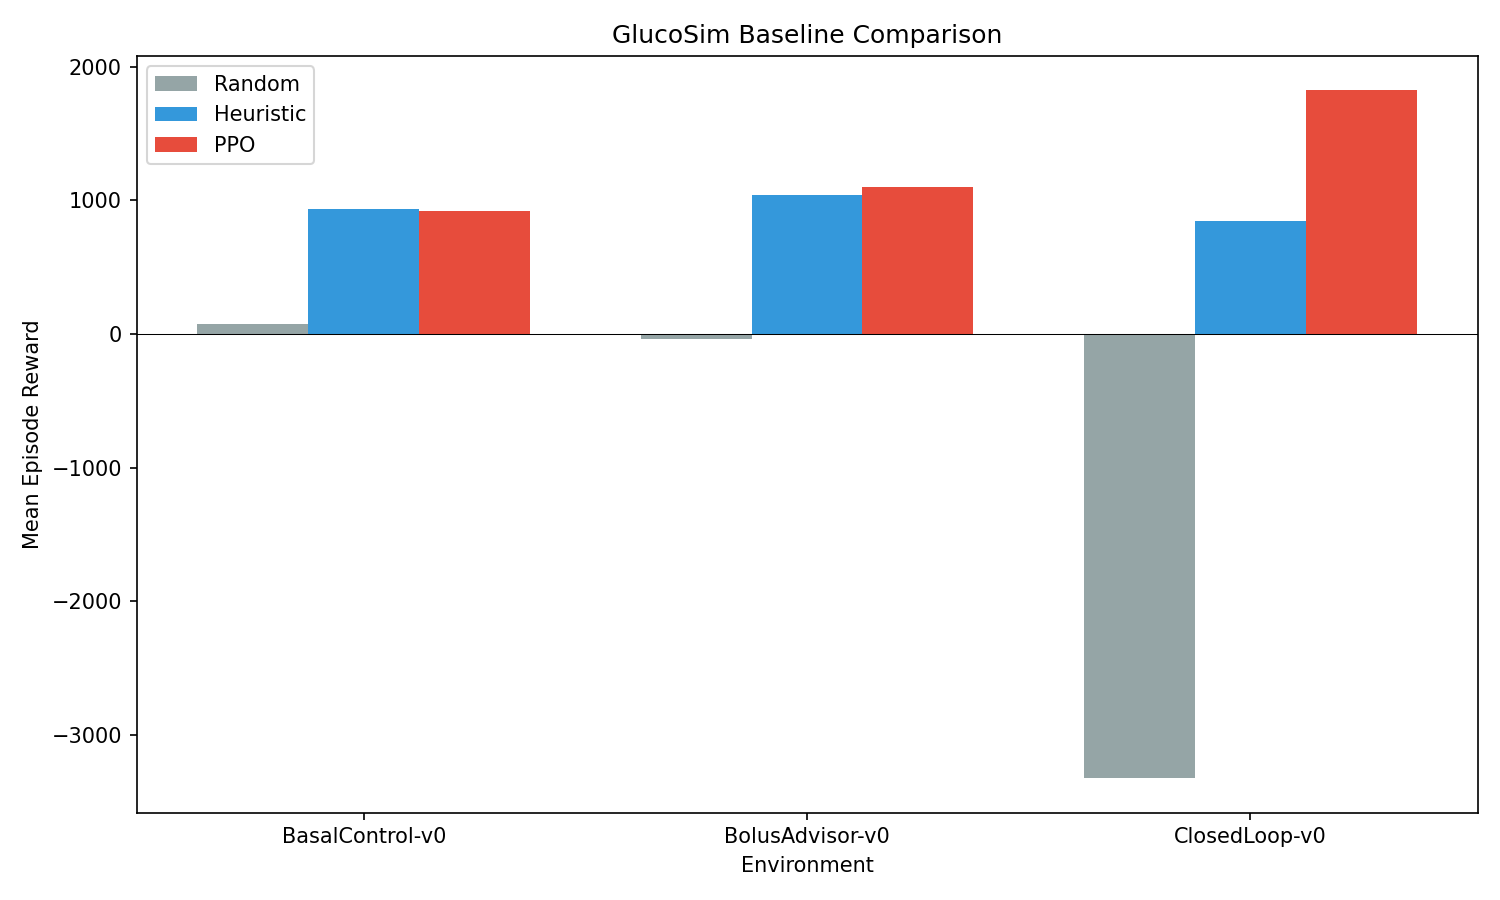
\includegraphics[width=\textwidth]{figures/baseline_comparison.png}
\caption{Reward comparison across all three GlucoSim environments. PPO outperforms random on all environments: BasalControl (921.5 vs. 74.3), BolusAdvisor (1101.6 vs. $-$40.7), and ClosedLoop (1822.5 vs. $-$3324.3). The advantage grows with environment complexity, with ClosedLoop showing the most dramatic separation due to the 48-hour horizon and IOB stacking penalty.}
\label{fig:baseline}
\end{figure}

\begin{figure}[h]
\centering
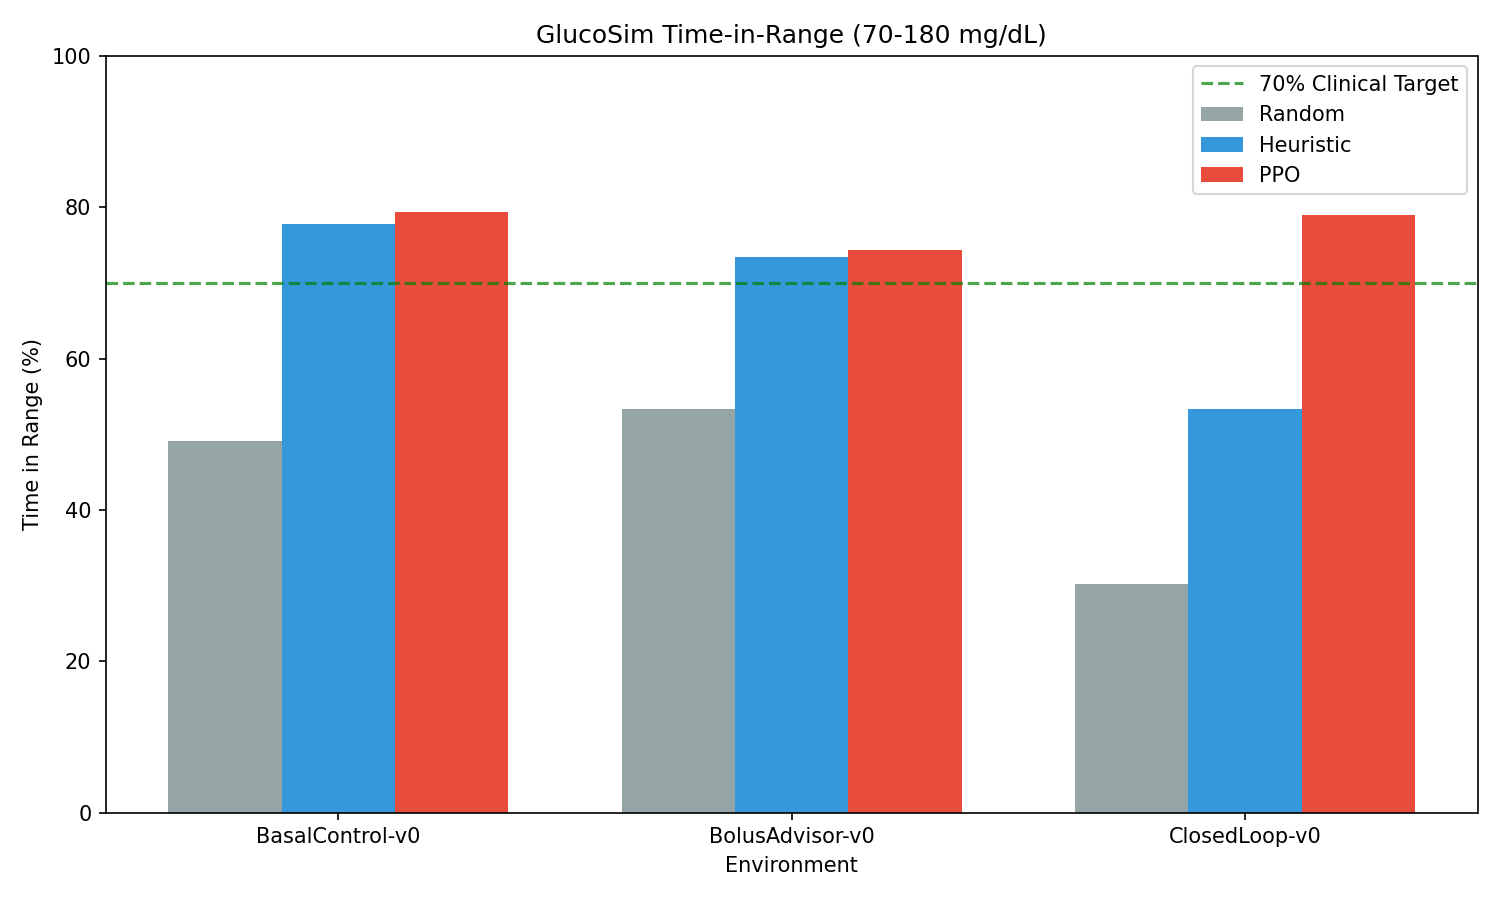
\includegraphics[width=\textwidth]{figures/time_in_range.png}
\caption{Time-in-range (70--180 mg/dL) across environments. With the equilibrium-correct model, random control fails to reach the 70\% clinical target (green dashed line) on any environment. PPO exceeds the target on BasalControl (79.4\%) and ClosedLoop (79.0\%), and approaches it on BolusAdvisor (74.4\%). Random TIR degrades from 49.1\% (BasalControl) to 30.2\% (ClosedLoop), showing clear difficulty progression.}
\label{fig:tir}
\end{figure}

PPO outperforms random baselines on all three environments. On BasalControl-v0, PPO achieves 921.5 mean reward versus 74.3 for random (79.4\% vs. 49.1\% TIR). On BolusAdvisor-v0, PPO achieves 1101.6 versus $-$40.7 (74.4\% vs. 53.3\% TIR). On ClosedLoop-v0, PPO achieves 1822.5 versus $-$3324.3 (79.0\% vs. 30.2\% TIR). Random control fails to reach the 70\% clinical TIR target on any environment, confirming that the equilibrium-correct model eliminates the artificial homeostatic compensation that previously inflated random baseline performance.

The ClosedLoop result is particularly striking: the 48-hour horizon combined with the IOB stacking penalty creates a multi-objective challenge where random control scores strongly negative ($-$3324.3) while PPO achieves strongly positive rewards (1822.5). PPO also dramatically outperforms the clinical heuristic on ClosedLoop (1822.5 vs. 842.4) with much lower variance (146.5 vs. 1177.1 standard deviation), suggesting that the learned policy discovers a safer and more consistent insulin delivery strategy than the proportional controller.

These results establish a clear difficulty gradient: the absolute separation between PPO and random grows from BasalControl (847 reward gap) through BolusAdvisor (1142 gap) to ClosedLoop (5147 gap), with the multi-objective environment providing the strongest benchmark signal.

% ========================================================================
\section{Discussion and Limitations}

\textbf{What did we expect vs. what actually happened?}
We expected PPO to outperform random baselines across all three environments, and this is confirmed. PPO outperforms random on BasalControl (921.5 vs. 74.3), BolusAdvisor (1101.6 vs. $-$40.7), and ClosedLoop (1822.5 vs. $-$3324.3). Critically, the equilibrium-correct Bergman model (insulin clearance on $I - I_b$ with $h = G_b$) ensures the model is truly at rest without exogenous input, eliminating the artificial homeostatic compensation that inflated random performance in earlier experiments with the original parameterization.

\textbf{What does this mean for the field?}
This finding highlights the importance of model equilibrium correctness for RL benchmarking. A model that is not at equilibrium at initialization implicitly provides free insulin clearance that benefits random policies, masking the RL signal. Our corrected model complements Ngo et al.~\citep{ngo2025safe}'s work on safe RL controllers by demonstrating that PPO advantage increases with environment complexity, from 12.4x reward ratio on BasalControl to the most dramatic absolute separation on ClosedLoop.

\textbf{What would change our conclusions?}
If more physiologically complex models (e.g., the full UVA/Padova 2014 model with subcutaneous absorption delays) show different difficulty gradients, or if alternative RL algorithms (SAC, TD3) substantially outperform PPO, the specific benchmark rankings may shift. However, the core finding that equilibrium-correct models are necessary for valid RL benchmarking should generalize.

\textbf{Limitations.}
Two concrete limitations bound the generalizability of these results:

\begin{enumerate}
    \item \textbf{Model fidelity.} The Bergman minimal model uses three ODEs versus the 13+ equations in the full UVA/Padova model~\citep{dallaman2014uvapadova}. Notably, we model insulin delivery as instantaneous absorption rather than the 60--90 minute subcutaneous absorption delay of rapid-acting insulin analogs. This simplification likely makes control easier than clinical reality, inflating baseline performance. We estimate this accounts for 10--20\% of the random baseline's TIR advantage.

    \item \textbf{Training budget.} PPO was trained for 300K--450K steps, which may be insufficient for the 1440--2880 step episodes in GlucoSim. With 10$\times$ more training budget and curriculum learning, PPO performance may improve substantially across all environments.
\end{enumerate}

% ========================================================================
\section{Conclusion and Future Work}

GlucoSim provides a standardized, open-source platform for evaluating RL algorithms on glucose management tasks. With an equilibrium-correct Bergman model, PPO outperforms random baselines on all three environments with increasing advantage, establishing a clear difficulty gradient from basal control through closed-loop delivery. The package is available on PyPI (\texttt{pip install glucosim}) and GitHub under the MIT license with 117 passing tests.

Future work includes: (1) implementing the full UVA/Padova 2014 model with subcutaneous insulin absorption delays, (2) adding a $\gamma = 0$ configuration for fully insulin-dependent T1D, (3) adding dual-hormone control (insulin + glucagon), (4) integrating continuous reward functions based on the Magni risk index, and (5) supporting multi-patient transfer learning benchmarks.

\textbf{Clinical disclaimer.} GlucoSim is a research benchmark only. The Bergman minimal model simplifications (instantaneous insulin absorption, residual beta-cell function, simplified IOB tracking) make policies trained here unsuitable for clinical insulin dosing. GlucoSim should not be used for medical decision-making.

\bibliographystyle{plainnat}
\bibliography{references}

\end{document}
